\documentclass[journal=jpccck,manuscript=article]{achemso}

\usepackage{amsmath}
\usepackage{siunitx}
\usepackage{booktabs}
\usepackage[T1]{fontenc}
\graphicspath{{figures/}}

\title{$\Delta$(ICOBI\textsubscript{antibonding}): A Fast Bond-Order-Based
Descriptor for the Kinetic Viability of Metastable Crystalline Compounds}

\author{Gilles Frapper}
\affiliation{IC2MP, UMR 7285 CNRS, Universit\'e de Poitiers, 4 rue Michel
Brunet, TSA 51106, 86073 Poitiers Cedex 9, France}
\email{gilles.frapper@univ-poitiers.fr}

\abbreviations{CSP,PES,COHP,ICOHP,COBI,ICOBI,DFT,AIMD,VBM}
\keywords{crystal structure prediction, chemical bonding analysis, LOBSTER,
COHP, COBI, metastability, kinetic stability, high-pressure chemistry}

\begin{document}

\begin{tocentry}
\centering
\textit{Table of Contents graphic to be inserted --- schematic of the
decomposition-into-elements reaction and the near-Fermi-level antibonding
window used to build $\Delta$(ICOBI\textsubscript{antibonding}).}
\end{tocentry}

\begin{abstract}
Crystal structure prediction routinely generates far more thermodynamically
metastable candidates than the phonon, elastic-constant, and \emph{ab
initio} molecular dynamics calculations needed for a full stability audit
can accommodate. We propose $\Delta$(ICOBI\textsubscript{antibonding}), the
change in the near-Fermi-level antibonding population of the Crystal
Orbital Bond Index upon a compound's decomposition into its elements, as an
inexpensive, single-static-calculation pre-screen for the kinetic viability
of such candidates, and test it, alongside its ICOHP-based counterpart, on
a Materials-Project-derived dataset of 597 unary and binary structures
(438--439 decomposition reactions) spanning stable, experimentally
realized metastable, and theoretical-only metastable compounds.
$\Delta$(ICOBI\textsubscript{antibonding}) correlates significantly with
formation energy ($\rho=-0.429$, $n=438$), significantly discriminates
experimentally realized from theoretical-only compounds (Fisher's exact
test, $p=2.4\times10^{-7}$), and, unlike every other ICOHP/ICOBI-derived
descriptor tested --- including the fully integrated reaction
$\Delta$(ICOHP) and the raw, non-reaction antibonding population --- survives
stratification by bonding type (metallic, ionic, covalent, mixed) in every
subgroup large enough to test. Because it requires no calculation beyond
the single static DFT+LOBSTER run already used to characterize a
compound's bonding, $\Delta$(ICOBI\textsubscript{antibonding}) offers a
practical route to concentrating the far more expensive stages of a
stability hierarchy on the metastable candidates most likely to correspond
to isolable compounds.
\end{abstract}

\section{Introduction}
\label{sec:intro}

Crystal structure prediction (CSP) --- and, in the molecular realm, the
closely related problem of conformer/isomer generation --- has become a
routine step in the computational discovery of new inorganic materials.
Evolutionary and random-sampling algorithms such as USPEX,\cite{oganov2006}
CALYPSO,\cite{wang2012} AIRSS,\cite{pickard2011} and XtalOpt\cite{zurek2021}
now explore compositional and configurational space largely unassisted,
generating, for a single target composition, dozens to hundreds of candidate
polymorphs, and, across a chemical system, an even larger set of
allotropes and stoichiometries.\cite{oganov2019} The traditional deliverable
of such a search is an energetic ranking: candidate structures are relaxed
at the density-functional-theory (DFT) level and ordered by total energy (or
enthalpy, under pressure) at 0~K, and, for a multi-component system, plotted
against composition to construct the thermodynamic convex hull --- the set of
compounds for which no combination of competing phases (elements or other
compounds of the same system) offers a lower-energy alternative at that
composition.\cite{ong2008,jain2013} Structures lying on the hull are, by
definition, thermodynamically stable at 0~K and $P=0$; every other stationary
point found by the search is \emph{metastable}, sitting some energy
$\Delta E_\text{hull}$ above it.

Being a stationary point of the potential energy surface (PES) --- a local
minimum surviving geometry relaxation --- is a necessary but far from
sufficient condition for a predicted compound to correspond to a real,
isolable material. A complete assessment of stability is, at minimum,
hierarchical over several physically distinct criteria: (i) \emph{energetic}
stability, position relative to the convex hull, already discussed above;
(ii) \emph{dynamical} stability, the absence of imaginary phonon frequencies
throughout the Brillouin zone, which rules out spontaneous symmetry-breaking
distortions and requires a full lattice-dynamics
calculation;\cite{togo2015} (iii) \emph{mechanical/elastic} stability, the
positive-definiteness of the elastic constant tensor (the Born--Huang
criteria), obtained from a set of finite strains and stress-tensor
evaluations;\cite{mouhat2014} (iv) \emph{thermal/kinetic} stability at finite
temperature, typically probed by \emph{ab initio} molecular dynamics (AIMD)
runs long enough to detect decomposition, amorphization, or a phase
transition;\cite{cohen2025} and, for open or multinary systems, (v)
\emph{chemical} stability against exchange with an external reservoir,
governed by the elemental chemical potentials and requiring, in principle,
its own grand-canonical convex-hull construction. These five criteria are
not redundant --- a compound can sit exactly on the convex hull and still be
dynamically or mechanically unstable, or conversely persist as a
long-lived metastable phase despite a positive $\Delta E_\text{hull}$ --- but
they are also not equally affordable. Energetic ranking requires one
static/relaxation calculation per candidate; phonon and elastic-constant
calculations require, respectively, a supercell (or density-functional
perturbation theory) treatment and a handful of strained-cell single points;
AIMD trajectories long enough to be diagnostic typically cost two to three
orders of magnitude more CPU time than a single static calculation. In a
CSP workflow that routinely produces $10^2$--$10^4$ candidate structures per
target composition, applying the full hierarchy to every metastable
candidate is computationally prohibitive, and in practice only a small,
pre-selected subset --- usually the lowest-energy candidates --- ever reaches
the phonon or AIMD stage.

This asymmetry between the number of thermodynamically metastable
stationary points a CSP search returns and the number that can be
subjected to a full stability audit motivates the search for cheap,
single-point descriptors able to pre-screen metastable candidates for their
likelihood of being experimentally realizable, deferring the expensive
criteria above to a much smaller shortlist. The conceptual basis for such a
pre-screen is not new: it is what Hoffmann and coworkers have termed the
\emph{viability} of a predicted compound --- the question of whether a
computed stationary point, however far above the convex hull, corresponds to
a structure that can actually be synthesized and persist, as opposed to one
that will spontaneously collapse back to its elements or to a
lower-lying phase the moment a synthesis is attempted.\cite{hoffmann1987,grochala2007}
Viability, in this sense, is fundamentally a kinetic property --- it concerns
the existence (or absence) of an activation barrier protecting the candidate
structure from decomposition --- rather than a thermodynamic one, and it is
precisely the criterion that energetic ranking and convex-hull position
cannot, on their own, resolve: many experimentally well-characterized
compounds sit measurably above the hull of their own chemical system, while
many hull-adjacent theoretical structures have never been made despite
repeated attempts.

A chemical-bonding-analysis route to this question can be built on the
Crystal Orbital Hamilton Population (COHP), which partitions the
band-structure energy into pairwise bonding (COHP~$<0$) and antibonding
(COHP~$>0$) contributions, and whose energy integral up to the Fermi level,
the ICOHP, quantifies the net strength of a given
bond.\cite{dronskowski1993,maintz2016} Summing ICOHP values over every bond
broken and formed in the decomposition of a compound into its constituent
elements yields a reaction descriptor, $\Delta$(ICOHP), whose sign we use
below to classify a compound's decomposition as \emph{endobondic}
(bond-breaking dominates, a kinetic barrier to decomposition is plausible) or
\emph{exobondic} (no such barrier is visible from bonding alone); this
bonding-based reasoning is attractive precisely because it is affordable:
unlike phonons or AIMD, it requires only a single self-consistent DFT
calculation per structure, post-processed with
LOBSTER,\cite{maintz2016,nelson2020} the program that projects
plane-wave/PAW wavefunctions onto a local atomic-orbital basis to recover
COHP and the closely related Crystal Orbital Bond Index
(COBI/ICOBI),\cite{muller2021,george2022} a dimensionless bond-order index
that follows the opposite sign convention (positive~=~bonding).

The present work builds on this bonding-based reasoning and asks a more
targeted question: rather than integrating the whole occupied COHP/COBI
trace, does restricting the integration to the antibonding population
confined to a narrow energy window just below the Fermi level (or the
valence-band maximum, for gapped compounds) --- the region most directly
implicated in Peierls- and Jahn--Teller-type electronic
instabilities --- yield a sharper, more broadly applicable viability
descriptor? We construct such a quantity for ICOBI,
$\Delta$(ICOBI\textsubscript{antibonding}), defined as the change, upon
decomposition of a compound into its elements, of the near-frontier
antibonding COBI population, and we validate it against a cohort of several
hundred compounds spanning the full spectrum from thermodynamically stable,
through experimentally realized but metastable, to theoretical
(never-synthesized) metastable structures, drawn from the Materials
Project.\cite{jain2013} The remainder of this article is organized as
follows: Section~\ref{sec:methods} details the dataset, the DFT+LOBSTER
computational protocol, and the precise definitions and sign conventions
used for every ICOHP/ICOBI-derived quantity; Sections~\ref{sec:results}
and~\ref{sec:discussion} (Results and Discussion) present the correlation of
$\Delta$(ICOBI\textsubscript{antibonding}) --- and, for comparison, of the
parent ICOHP-based descriptors --- against thermodynamic stability targets
and against a binary experimental/theoretical viability label, stratified by
bonding character; Section~\ref{sec:conclusion} concludes.

\section{Methodology}
\label{sec:methods}

\subsection{Dataset}
\label{sec:dataset}

Candidate compounds were drawn from the Materials Project
database\cite{jain2013} by querying unary and binary chemical systems,
restricted to non-magnetic structures (absolute total magnetization
$\leq 0.01~\mu_\text{B}$ per formula unit --- computed directly from the
stored magnetic moments rather than from the Materials Project's categorical
\texttt{magnetic\_ordering} field, which is unassigned for the large
majority of entries) and excluding $f$-block elements. The final dataset
combines three complementary selection tracks totaling 597 structures: (i) a
first, broadly representative set (\num{20} atoms/cell or fewer, balanced
across stability classes, capped at two entries per chemical system to
maximize elemental diversity over redundant polymorphs); (ii) a second set
(\num{40} atoms/cell or fewer) specifically targeting additional elemental
references, off-equilibrium polymorphs (high-pressure phases, allotropes),
and alkali/alkaline-earth binaries against N, O, F, P, S, and Cl, chosen to
build genuine same-composition polymorph groups and to probe descriptor
behavior far from equilibrium; and (iii) a third, deliberately adversarial
set of 45 binary compounds pairing an experimentally known compound sitting
farthest above the convex hull of its chemical system with one to three
theoretical polymorphs of the same formula lying even farther above the
hull, targeting the stability edge cases where a viability descriptor is
most needed and most likely to fail. Each entry carries the Materials
Project stability label (on-hull, experimentally observed metastable, or
theoretical-only metastable, the last serving as the closest available
proxy for a compound that has been searched for but never made) and,
where available, \texttt{formation\_energy\_per\_atom} and
\texttt{energy\_above\_hull} as continuous thermodynamic targets.

\subsection{Electronic-Structure and Bonding-Analysis Protocol}
\label{sec:dft-lobster}

All structures were treated with an identical computational template to
avoid introducing system-dependent methodological bias. Static
(single-point) DFT calculations were performed with the Vienna Ab initio
Simulation Package (VASP),\cite{kresse1996} using the projector
augmented-wave (PAW) method\cite{blochl1994,kresse1999} with the PAW-PBE
potentials recommended by \texttt{pymatgen}'s \texttt{MPRelaxSet}, the PBE
generalized-gradient exchange--correlation functional,\cite{perdew1996}
symmetry explicitly disabled (\texttt{ISYM=$-1$}) to avoid artifacts in the
subsequent bonding projection, and non-spherical gradient corrections
enabled (\texttt{LASPH=.TRUE.}). The number of bands was set, per compound,
from the number of local orbitals required by the LOBSTER basis rather than
from a fixed multiplier, and basis-function assignment for each species was
obtained programmatically rather than by parsing POTCAR headers directly, to
avoid failures on potentials not recognized by hash in the local mirror.
Chemical-bonding analysis was then performed with LOBSTER
5.1.1,\cite{maintz2016,nelson2020} projecting the converged VASP wavefunction
onto the \texttt{pbeVaspFit2015} local basis, with a common COHP/COBI
integration window from $-35$ to $+5$~eV around the Fermi level, bond
detection by interatomic distance from 0.1 to 6.0~\AA{} (orbital-resolved),
and 0.05~eV Gaussian smearing. This identical template was applied to every
structure in the dataset (Section~\ref{sec:validation-methods} details the
internal quality-control diagnostics used to screen the resulting
ICOHP/ICOBI output before any descriptor was computed from it).

\subsection{ICOHP and ICOBI: Definitions and Sign Conventions}
\label{sec:icohp-icobi-def}

The Crystal Orbital Hamilton Population, COHP($E$), resolves the
band-structure energy of a pair of atoms into an energy-dependent bonding
(negative) and antibonding (positive) contribution.\cite{dronskowski1993} Its
integral up to the Fermi level, the ICOHP, is by convention negative for a
net bonding interaction and positive for a net antibonding one, and is
reported in eV. The Crystal Orbital Bond Index, COBI($E$), and its integral
ICOBI, are constructed analogously but derived directly from the density
matrix rather than from the band-structure energy, and quantify covalent
bond order rather than bond strength;\cite{muller2021} critically, ICOBI
follows the \emph{opposite} sign convention to ICOHP --- positive ICOBI
denotes a net bonding interaction, as for the older Crystal Orbital Overlap
Population (COOP) --- so that the antibonding contribution to ICOBI is its
\emph{negative}, not positive, part. This distinction, verified numerically
against \texttt{ICOBILIST.lobster} output, is essential whenever ICOHP- and
ICOBI-derived descriptors are combined or compared, and every quantity
defined below states explicitly which convention it follows.

Two extensive per-compound aggregates are used as a baseline throughout this
work: \texttt{icohp\_sum}/\texttt{icobi\_sum}, summing every symmetrically
inequivalent bond label reported by LOBSTER within its detection window
(each periodic bond counted once, irrespective of the number of equivalent
directions), and the corresponding intensive per-bond averages,
\texttt{icohp\_mean}/\texttt{icobi\_mean}. No coordination-shell filtering is
applied to these baseline aggregates, so that every compound in the dataset
is treated identically regardless of its local coordination chemistry.

\subsection{Reaction $\Delta$(ICOHP) and the Endobondic/Exobondic
Classification}
\label{sec:delta-icohp}

For the decomposition of a compound into its constituent elements
(``case-1'' reactions in the sense of Bartel \emph{et al.},\cite{bartel2019}
i.e. reactions whose products are exclusively elemental references), the
reaction descriptor is defined, following the products$-$reactants
thermochemical convention, as
\begin{equation}
  \Delta(\text{ICOHP}) \;=\; \sum_{\text{products}} \nu_i\, \text{ICOHP}_i
  \;-\; \sum_{\text{reactants}} \nu_j\, \text{ICOHP}_j ,
  \label{eq:delta-icohp}
\end{equation}
with $\nu$ the stoichiometric coefficients of the balanced reaction, computed
in three normalizations (per formula unit, per transferred atom --- the
normalization used throughout unless stated otherwise --- and, diagnostically
only, per bond, which is not strictly conserved between differently-bonded
structures). A positive $\Delta$(ICOHP) (\emph{endobondic}) indicates that
breaking the compound's bonds costs more, in ICOHP terms, than the bonds of
the free elements recover --- a signature compatible with a kinetic barrier
protecting the compound from decomposition; a negative value
(\emph{exobondic}) indicates no such barrier is visible from bonding alone.
The sign of
$\Delta$(ICOHP) is combined with the sign of the thermodynamic driving force
for decomposition ($\Delta E$, from \texttt{formation\_energy\_per\_atom}) to
assign each compound a three-way viability label: a compound is classified
\texttt{UNSTABLE\_NONEXISTENT} only if decomposition into elements is
\emph{both} exobondic \emph{and} thermodynamically favorable; a compound with
$\Delta E \geq 0$ or an endobondic decomposition is classified
\texttt{STABLE\_ON\_HULL} or \texttt{METASTABLE\_VIABLE} as appropriate. This
combined label, rather than the sign of $\Delta$(ICOHP) in isolation, is the
target used to test experimental/theoretical discrimination in
Section~\ref{sec:results}.

\subsection{Near-Frontier Antibonding Population and Its Reaction
$\Delta$}
\label{sec:antibonding-def}

A distinct construction targets not the total bonding integrated over the
whole occupied manifold, but specifically the antibonding population
confined to a narrow window adjacent to the frontier orbitals, by analogy
with electronically driven (Peierls/Jahn--Teller-type) instabilities, for
which only occupied antibonding character near $E_\text{F}$ is expected to
be destabilizing. For ICOHP, this quantity integrates only the antibonding
part of the COHP trace (COHP~$>0$) over a one-sided energy window
$(E_\text{ref}-\Delta E,\; E_\text{ref}]$, where $E_\text{ref}$ is the Fermi
level for metallic compounds (\texttt{is\_metal} = true) or the valence-band
maximum for gapped compounds, and $\Delta E \in \{0.5, 1.0, 2.0\}$~eV, with
$\Delta E = 1.0$~eV as the primary window reported here. The identical
construction is applied to the COBI trace, reading from
\texttt{COBICAR.lobster}/\texttt{ICOBILIST.lobster} instead of
\texttt{COHPCAR.lobster}/\texttt{ICOHPLIST.lobster}; because ICOBI's sign
convention is the mirror image of ICOHP's (Section~\ref{sec:icohp-icobi-def}),
the antibonding part of ICOBI is taken as its \emph{negative} region, not its
positive one --- a deliberate mirror-image truncation, not a copy of the
ICOHP procedure. Both quantities are computed from LOBSTER's own
pre-aggregated, per-bond-weighted ``average'' COHP/COBI trace rather than
from a sum over discrete bond pairs, so that, unlike the aggregates of
Section~\ref{sec:icohp-icobi-def}, no coordination-shell or bond-pair
filtering enters their definition; only the energy window near
$E_\text{ref}$ does. Both are reported in raw units (eV for the ICOHP-based
quantity, dimensionless for the ICOBI-based one, though neither is literally
an energy or a bond order once restricted to a sub-window) and normalized by
the total occupied ICOHP (respectively ICOBI) magnitude at the same
$E_\text{ref}$.

Because this near-frontier antibonding population is, by construction, an
intensive quantity (a per-bond average over the whole occupied trace, with
no natural extensive decomposition into individual bonds), its reaction
counterpart cannot be built by the same stoichiometric summation as
Eq.~\ref{eq:delta-icohp}. Instead, for a compound decomposing into elements
$k$ with atomic fractions $x_k$,
\begin{equation}
  \Delta(\text{antibonding}) \;=\; \sum_{k} x_k\,\text{antibonding}_k
  \;-\; \text{antibonding}_\text{compound} ,
  \label{eq:delta-antibonding}
\end{equation}
again in the products$-$reactants convention, with
\texttt{antibonding}$_k$/\texttt{antibonding}$_\text{compound}$ evaluated
either on the ICOHP-based or the ICOBI-based near-frontier population,
yielding two descriptors, $\Delta$(ICOHP\textsubscript{antibonding}) and
$\Delta$(ICOBI\textsubscript{antibonding}) respectively; the latter is the
central descriptor of this work. A compound whose formation \emph{reduces}
near-frontier antibonding character relative to its constituent elements
corresponds to $\Delta(\text{antibonding}) > 0$.

\subsection{Bonding-Type Classification}
\label{sec:bondtype}

Because the strength and interpretation of ICOHP/ICOBI-derived quantities
depend on bonding character, every compound and element was additionally
assigned to one of five categories --- metallic, ionic, covalent, mixed
(Zintl-type), or unclassified --- used throughout as a stratification
variable rather than as an end in itself. Two independent classification
routes were compared. The first is a composition-based heuristic using
only elemental identity and the \texttt{is\_metal} flag: \texttt{is\_metal}
compounds with $\geq2$ elements and no anion-forming element present
(halogens, O, N, S, Se, Te, H, C, P, As, B) are labeled metallic; among
the remainder, an alkali/alkaline-earth element co-occurring with a
halogen or O gives ionic, and a covalent-forming element (B, C, Si, Ge,
N, P, As, Al, Ga, In, Sn, Pb, S, Se, Te) with no alkali/alkaline-earth
present gives covalent; all other compositions are left unclassified.
The second, used for every stratified result reported below, is built
directly from the LOBSTER output of Section~\ref{sec:icohp-icobi-def}:
\texttt{is\_metal} again gives metallic; otherwise the compound's
\emph{dominant} species pair (highest mean ICOBI over its first
coordination shell, among all pairs LOBSTER reports) is compared against
a threshold calibrated as the midpoint between the median dominant-pair
ICOBI of compounds the first (composition-based) route already labels
ionic and those it labels covalent (0.5315 in the current dataset),
giving ionic below and covalent at or above that value; a compound whose
\emph{homoatomic} pair (e.g. N--N, P--P, S--S) reaches the threshold
while a distinct, weaker \emph{heteroatomic} pair is also present ---
the Zintl--Klemm signature of a covalent polyanion loosely bound to a
separate cation --- is assigned to the mixed category instead, since
forcing a single ionic/covalent label would misrepresent it. First
coordination shells, where used (this classification and the validation
reactions of Section~\ref{sec:validation-methods} only), are delimited
by an adaptive, self-calibrating rule on the sorted bond-distance
spectrum of each species pair (cutting at the first gap exceeding
2.5$\times$ the largest gap seen so far within the putative shell),
rather than by a fixed distance cutoff.

\subsection{Statistical Analysis}
\label{sec:stats}

Because no linear relationship is assumed \emph{a priori} between any
ICOHP/ICOBI-derived descriptor and a thermodynamic stability target,
association is quantified throughout by Spearman rank correlation ($\rho$)
against \texttt{formation\_energy\_per\_atom} and
\texttt{energy\_above\_hull}, computed both over the full dataset and within
each bonding-type/metallicity subgroup of Section~\ref{sec:bondtype}; any
subgroup with fewer than 15 members is reported but explicitly flagged as
underpowered, never presented without that caveat. Discrimination between
experimentally realized and theoretical-only (never synthesized) compounds
is tested with Fisher's exact test on the corresponding $2\times2$
contingency table (endobondic/exobondic, or descriptor sign, versus
experimental/theoretical status) and, for the underlying continuous
descriptor, with a Mann--Whitney $U$ test; the same pair of tests is applied
to the combined \texttt{ViabilityLabel} of Section~\ref{sec:delta-icohp}
against experimental/theoretical status, and to
$\Delta$(ICOHP\textsubscript{antibonding})/$\Delta$(ICOBI\textsubscript{antibonding})
against a binary viable/non-viable split derived from the same label.

\subsection{Quality Control}
\label{sec:validation-methods}

Before any descriptor was computed, every LOBSTER run was screened with two
internal diagnostics available from its own output: the fraction of
$k$-points for which the projected local basis fails to reach
orthonormalization (\texttt{lobsterout}) and the maximum deviation reported
in \texttt{bandOverlaps.lobster}, an established red-flag threshold of 0.1
being used to separate a numerically trustworthy projection from a
pathological one. A systematic sweep of the full dataset under a
conservative combined criterion (100\% $k$-point failure \emph{and} a
band-overlap deviation $>0.5$ \emph{and} a robust $z$-score $>10$ on the
resulting $\Delta$(ICOHP)) is reported in Section~\ref{sec:limits}.

\section{Results and Discussion}
\label{sec:results}
\label{sec:discussion}

\subsection{Dataset and Bonding-Type Classification}
\label{sec:res-dataset}

The final dataset (Section~\ref{sec:dataset}) comprises 597 VASP+LOBSTER
calculations, of which 588 yield a usable ICOHP/ICOBI record after quality
control (Section~\ref{sec:limits}); 439 of these participate in at least one
decomposition-into-elements (case-1) reaction and therefore carry a
$\Delta$(ICOHP)/$\Delta$(antibonding) value. The bonding-based classification
of Section~\ref{sec:bondtype} assigns 372 compounds/elements as metallic, 98
as ionic, 56 as covalent, and 62 as mixed (Zintl-type), with every entry
receiving a verdict. Where the composition-based heuristic also renders a
verdict, the two classifications agree in 276/311 cases (88.7\%); the
disagreements concentrate in 19 compounds the heuristic calls ionic or
covalent but whose dominant homoatomic bond (e.g. a polyanionic N--N, P--P,
or S--S contact) the bonding-based route instead flags as mixed, and in a
further 16 ionic/covalent swaps. Because the bonding-based classification
also resolves the 277 compounds (47\%) the composition-only heuristic leaves
unclassified --- chiefly alkali/alkaline-earth pairs with N, P, or S not
covered by a fixed anion list --- it is used throughout as the
stratification variable below.

\subsection{Baseline Correlations}
\label{sec:res-baseline}

Before turning to the near-frontier antibonding descriptors that are the
focus of this work, three simpler ICOHP/ICOBI-derived quantities set a
baseline. The classic per-compound aggregates (\texttt{icohp\_sum},
\texttt{icohp\_min}) correlate weakly or not at all with
$E_\text{hull}$ (Spearman $\rho = 0.032$ and $0.093$, $n=186$, both
non-significant; a weak but significant signal appears only in the metallic
subgroup, $\rho=0.223$, $p=0.037$). The reaction descriptor $\Delta$(ICOHP)
(Eq.~\ref{eq:delta-icohp}) does better: pooled over 510--514 case-1
reactions, $\rho=0.295$ against \texttt{formation\_energy\_per\_atom}
($p\approx0$) but only $\rho=-0.056$ ($p=0.20$, not significant) against
\texttt{energy\_above\_hull}. The endobondic/exobondic sign of
$\Delta$(ICOHP) alone discriminates experimentally realized from
theoretical-only compounds (Fisher's exact test, odds ratio $1.81$,
$p=0.0054$, endobondic decompositions being $\sim$1.8$\times$ more frequent
among experimentally realized compounds); combining that sign with the
thermodynamic driving force into the three-way \texttt{ViabilityLabel} of
Section~\ref{sec:delta-icohp} sharpens this considerably (odds ratio
$6.0$, $\chi^2=59.0$, $p=1.6\times10^{-14}$ on the collapsed viable/not-viable
split) --- of 188 experimentally realized compounds whose decomposition is
exobondic, only 26 are in fact predicted non-viable, because for the other
162 that decomposition is thermodynamically unfavorable despite lacking a
bonding-based barrier. This large gap between the sign-only test and the
combined label is itself instructive: sign alone is a real but partial
signal, and it is the combination with thermodynamics that carries most of
the discriminating power in the ICOHP-integrated picture.

The raw near-frontier antibonding population (Section~\ref{sec:antibonding-def},
not yet a reaction quantity) correlates with \texttt{formation\_energy\_per\_atom}
at $\rho=-0.155$ ($p=1.8\times10^{-4}$, $n=579$) for its ICOHP-based version
--- a counter-intuitive sign, since more occupied antibonding character near
$E_\text{F}$ is here associated with a \emph{more}, not less, stable
formation --- and at $\rho=+0.231$ ($n=579$) for its ICOBI-based version,
i.e. the naively expected direction. Table~\ref{tab:antibonding-icohp-icobi}
compares the two, overall and by bonding-type subgroup.

\begin{table}[htbp]
\centering
\caption{Spearman correlations of the raw near-frontier antibonding
population (not a reaction quantity) against
\texttt{formation\_energy\_per\_atom}, ICOHP- versus ICOBI-based, same
underlying population ($n=588$; $\Delta E = 1.0$~eV window).}
\label{tab:antibonding-icohp-icobi}
\begin{tabular}{@{}lrrrr@{}}
\toprule
Subgroup & $n$ & $\rho$ (ICOHP) & $n$ & $\rho$ (ICOBI) \\
\midrule
all              & 579 & $-0.155^{***}$ & 579 & $+0.231^{***}$ \\
covalent         & 54  & $-0.046$       & 54  & $+0.113$ \\
ionic            & 96  & $-0.196$       & 96  & $+0.162$ \\
metallic         & 367 & $+0.056$       & 367 & $+0.120^{*}$ \\
mixed            & 62  & $-0.538^{***}$ & 62  & $+0.025$ \\
\bottomrule
\end{tabular}
\vspace{0.1cm}
\\{\footnotesize $^{*}p<0.05$; $^{***}p<0.001$; no star = not significant.}
\end{table}

Two observations motivate restricting attention, in what follows, to the
\emph{reaction} $\Delta$ of this antibonding population rather than its raw
value. First, the ICOHP- and ICOBI-based versions of the raw population run
in \emph{opposite} directions overall, a direct consequence of their
opposite sign convention (Section~\ref{sec:icohp-icobi-def}) rather than of
any disagreement in the underlying physics. Second, only the mixed
(Zintl-type) subgroup survives stratification for either quantity at this
scale; a stratified result reported for the covalent subgroup at a smaller
sample size in earlier stages of this project did not survive once the
sample grew to $n=54$ ($\rho=-0.046$, $p=0.74$), underscoring that any
single-stratum result must be re-checked as a dataset grows rather than
taken as settled.

\subsection{$\Delta$(Antibonding) of the Decomposition Reaction}
\label{sec:res-delta-antibonding}

For a case-1 reaction, $\Delta$(antibonding) (Eq.~\ref{eq:delta-antibonding})
was computed for 438--439 reactions. Table~\ref{tab:delta-antibonding}
reports its correlation with both thermodynamic targets, for the ICOHP- and
ICOBI-based versions side by side.

\begin{table}[htbp]
\centering
\caption{Spearman correlations, $\Delta$(antibonding) of the
decomposition-into-elements reaction ($n=438$--439).}
\label{tab:delta-antibonding}
\begin{tabular}{@{}lrrr@{}}
\toprule
Descriptor & Target & $n$ & $\rho$ \\
\midrule
$\Delta$(ICOHP\textsubscript{antibonding}) & formation energy/atom & 438 & $-0.6225^{***}$ \\
$\Delta$(ICOBI\textsubscript{antibonding}) & formation energy/atom & 438 & $-0.4292^{***}$ \\
$\Delta$(ICOHP\textsubscript{antibonding}) & energy above hull     & 438 & $-0.1734^{***}$ \\
$\Delta$(ICOBI\textsubscript{antibonding}) & energy above hull     & 438 & $-0.1215^{*}$ \\
\bottomrule
\end{tabular}
\vspace{0.1cm}
\\{\footnotesize $^{*}p<0.05$; $^{***}p<0.001$.}
\end{table}

\begin{figure}[htbp]
\centering
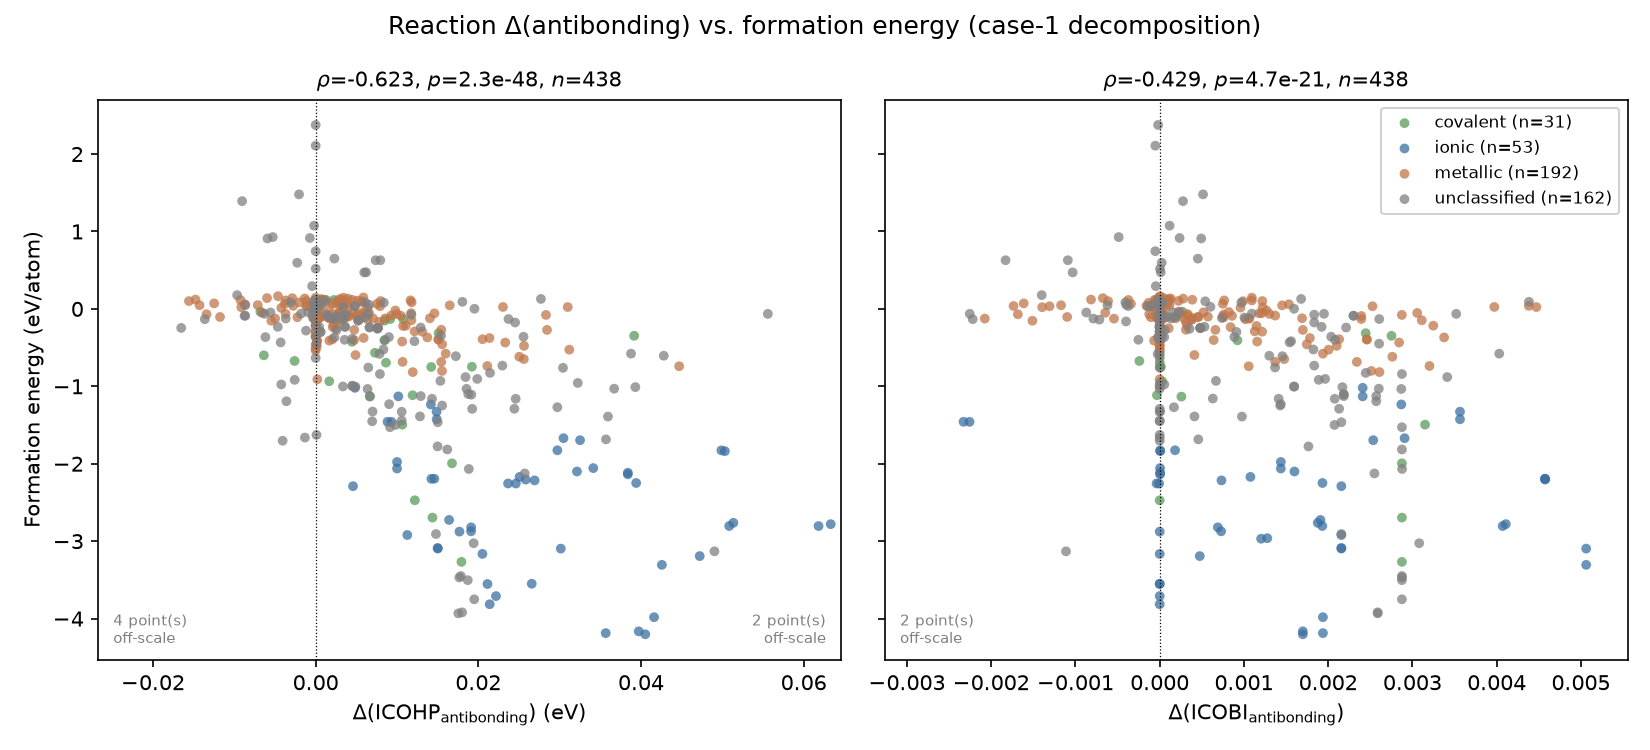
\includegraphics[width=\textwidth]{delta_antibonding_vs_formation_energy.png}
\caption{Formation energy per atom versus $\Delta$(ICOHP\textsubscript{antibonding})
(left) and $\Delta$(ICOBI\textsubscript{antibonding}) (right) of the
decomposition-into-elements reaction, colored by bond type ($n=438$).
Spearman $\rho$ and $p$ (title of each panel) are computed on the full
population; the $x$-axis is clipped to the 1st--99th percentile of each
descriptor so that a small number of extreme-magnitude compounds do not
compress the rest of the population, with the count of clipped points
noted in-panel. The ionic subgroup (blue) drives most of the visible
trend, consistent with Table~\ref{tab:delta-antibonding-stratified}.}
\label{fig:delta-antibonding-vs-formation-energy}
\end{figure}

Two features distinguish this reaction-level construction from the raw
population of Section~\ref{sec:res-baseline}. First,
$\Delta$(ICOHP\textsubscript{antibonding}) is, at $\rho=-0.6225$, the
strongest continuous correlation identified anywhere in this work ---
stronger than either the raw antibonding population or the fully integrated
reaction $\Delta$(ICOHP) of Section~\ref{sec:res-baseline}
($\rho=0.295$; note the reaction-ICOHP figure is reported in the
products$-$reactants convention of \texttt{reaction\_icohp.py}, opposite in
sign to but equal in magnitude to the $\Delta$(ICOHP) convention of
Eq.~\ref{eq:delta-icohp}). Second, and more directly relevant to the present
focus, $\Delta$(ICOBI\textsubscript{antibonding}) --- the central descriptor
of this work --- now runs in the \emph{same} direction as its ICOHP
counterpart ($\rho=-0.4292$, both negative), even though the raw,
non-reaction antibonding populations they are built from run in opposite
directions (Table~\ref{tab:antibonding-icohp-icobi}). Taking the reaction
$\Delta$, i.e. referencing each compound's near-frontier antibonding
character against the atomic-fraction-weighted average of its own elements
rather than reading it in isolation, thus removes the sign ambiguity between
the ICOHP and ICOBI bond-order conventions and leaves a consistent, physically
interpretable picture: \emph{a compound whose formation reduces near-frontier
antibonding character relative to its constituent elements
($\Delta > 0$ in our convention, i.e. a negative correlation with formation
energy since more negative formation energies are more stable) is more
likely to be thermodynamically favorable.}

\begin{figure}[htbp]
\centering

\includegraphics[width=0.85\textwidth]{icohp_vs_icobi_antibonding_comparison.png}
\caption{$\Delta$(ICOHP\textsubscript{antibonding}) and
$\Delta$(ICOBI\textsubscript{antibonding}) of the decomposition-into-elements
reaction, both plotted against \texttt{formation\_energy\_per\_atom}
($n=438$).}
\label{fig:icohp-icobi-comparison}
\end{figure}

\subsection{Stratification by Bonding Type}
\label{sec:res-stratification}

Table~\ref{tab:delta-antibonding-stratified} tests whether the pooled
correlations above survive once conditioned on the bonding-type
classification of Section~\ref{sec:res-dataset}.

\begin{table}[htbp]
\centering
\caption{Spearman correlations, $\Delta$(antibonding) against
\texttt{formation\_energy\_per\_atom}, by bonding-type subgroup ($n=438$
pooled).}
\label{tab:delta-antibonding-stratified}
\begin{tabular}{@{}lrrrr@{}}
\toprule
Subgroup & $n$ & $\rho$ ($\Delta$ICOHP\textsubscript{ab}) & $n$ & $\rho$ ($\Delta$ICOBI\textsubscript{ab}) \\
\midrule
all              & 438 & $-0.6225^{***}$ & 438 & $-0.4292^{***}$ \\
covalent         & 29  & $-0.6956^{***}$ & 29  & $-0.7750^{***}$ \\
ionic            & 89  & $-0.6301^{***}$ & 89  & $-0.2258^{*}$ \\
metallic         & 288 & $-0.4359^{***}$ & 288 & $-0.3602^{***}$ \\
mixed            & 32  & $-0.6394^{***}$ & 32  & $-0.8397^{***}$ \\
\texttt{is\_metal}=False & 150 & $-0.6466^{***}$ & 150 & $-0.4128^{***}$ \\
\texttt{is\_metal}=True  & 288 & $-0.4359^{***}$ & 288 & $-0.3602^{***}$ \\
\bottomrule
\end{tabular}
\vspace{0.1cm}
\\{\footnotesize $^{*}p<0.05$; $^{***}p<0.001$; no star = not significant.}
\end{table}

This is, to our knowledge, the only result in this study --- and, notably,
the only one for either the ICOHP- or the ICOBI-based version --- that
survives \emph{every} stratification tested, covalent through metallic,
$\texttt{is\_metal}$ on both sides, all significant at $p<0.001$. By
contrast, the raw antibonding population retains only two surviving strata
(mixed, \texttt{is\_metal}=False; Section~\ref{sec:res-baseline}) and the
fully integrated reaction $\Delta$(ICOHP) survives on \texttt{bond\_type}
but not within the majority metallic stratum
(Section~\ref{sec:res-baseline}). $\Delta$(ICOBI\textsubscript{antibonding})
reaches its strongest single-stratum value on the mixed (Zintl-type)
subgroup ($\rho=-0.840$), a category whose bonding --- a strongly covalent
homoatomic polyanion alongside a much weaker heteroatomic, more ionic
contact --- is precisely the kind of chemically heterogeneous bonding
picture a single pooled descriptor is most likely to average away; that both
$\Delta$(antibonding) quantities instead sharpen \emph{within} this subgroup
suggests the near-frontier restriction is tracking a genuinely local
electronic feature rather than a composition-driven confound. The smaller
subgroups here (covalent, $n=29$; mixed, $n=32$) fall below this project's
own $n=15$ significance-reporting floor only in the sense of statistical
power, not in significance itself --- both remain significant at
$p<0.001$ --- but should still be read as provisional pending a larger,
independent sample.

\subsection{Discrimination of Experimentally Realized from Theoretical-Only
Compounds}
\label{sec:res-viability}

The continuous correlations above test agreement with a thermodynamic
target; a stricter and more directly relevant test is whether
$\Delta$(antibonding) discriminates compounds that have actually been made
from theoretical-only candidates that, despite comparable or lower
$E_\text{hull}$, have never been synthesized. Using the same
\texttt{ViabilityLabel} convention as Section~\ref{sec:res-baseline}
(viable~$=$~\texttt{STABLE\_ON\_HULL}~$\cup$~\texttt{METASTABLE\_VIABLE},
not viable~$=$~\texttt{UNSTABLE\_NONEXISTENT}), Table~\ref{tab:viability-antibonding}
reports Mann--Whitney $U$ on the continuous
$\Delta$(ICOHP\textsubscript{antibonding}) and Fisher's exact test on its
sign, by subgroup ($n_\text{total}=434$).

\begin{table}[htbp]
\centering
\caption{$\Delta$(ICOHP\textsubscript{antibonding}) versus viability, by
subgroup.}
\label{tab:viability-antibonding}
\begin{tabular}{@{}lrrrrr@{}}
\toprule
Subgroup & $n$ viable & $n$ not viable & Mann--Whitney $p$ & Fisher OR & Fisher $p$ \\
\midrule
all                       & 329 & 105 & $6.7\times10^{-12\,***}$ & 3.49 & $2.4\times10^{-7\,***}$ \\
\texttt{bond\_type}=metallic & 125 & 65  & $0.0028^{**}$            & 2.20 & $0.021^{*}$ \\
\texttt{is\_metal}=True      & 187 & 99  & $6.7\times10^{-5\,***}$  & 2.38 & $0.00099^{***}$ \\
\texttt{is\_metal}=False     & 142 & 6   & $0.012^{*}$              & 7.88 & $0.028^{*}$ \\
\bottomrule
\end{tabular}
\vspace{0.1cm}
\\{\footnotesize $^{*}p<0.05$; $^{**}p<0.01$; $^{***}p<0.001$. Median
$\Delta$(ICOHP\textsubscript{antibonding})$= 0.0067$~eV (viable) vs.\
$3.2\times10^{-6}$~eV (not viable), all-subgroup. \texttt{bond\_type}=covalent
(3 non-viable) and \texttt{bond\_type}=ionic (1 non-viable) are too small to
test.}
\end{table}

\begin{figure}[htbp]
\centering
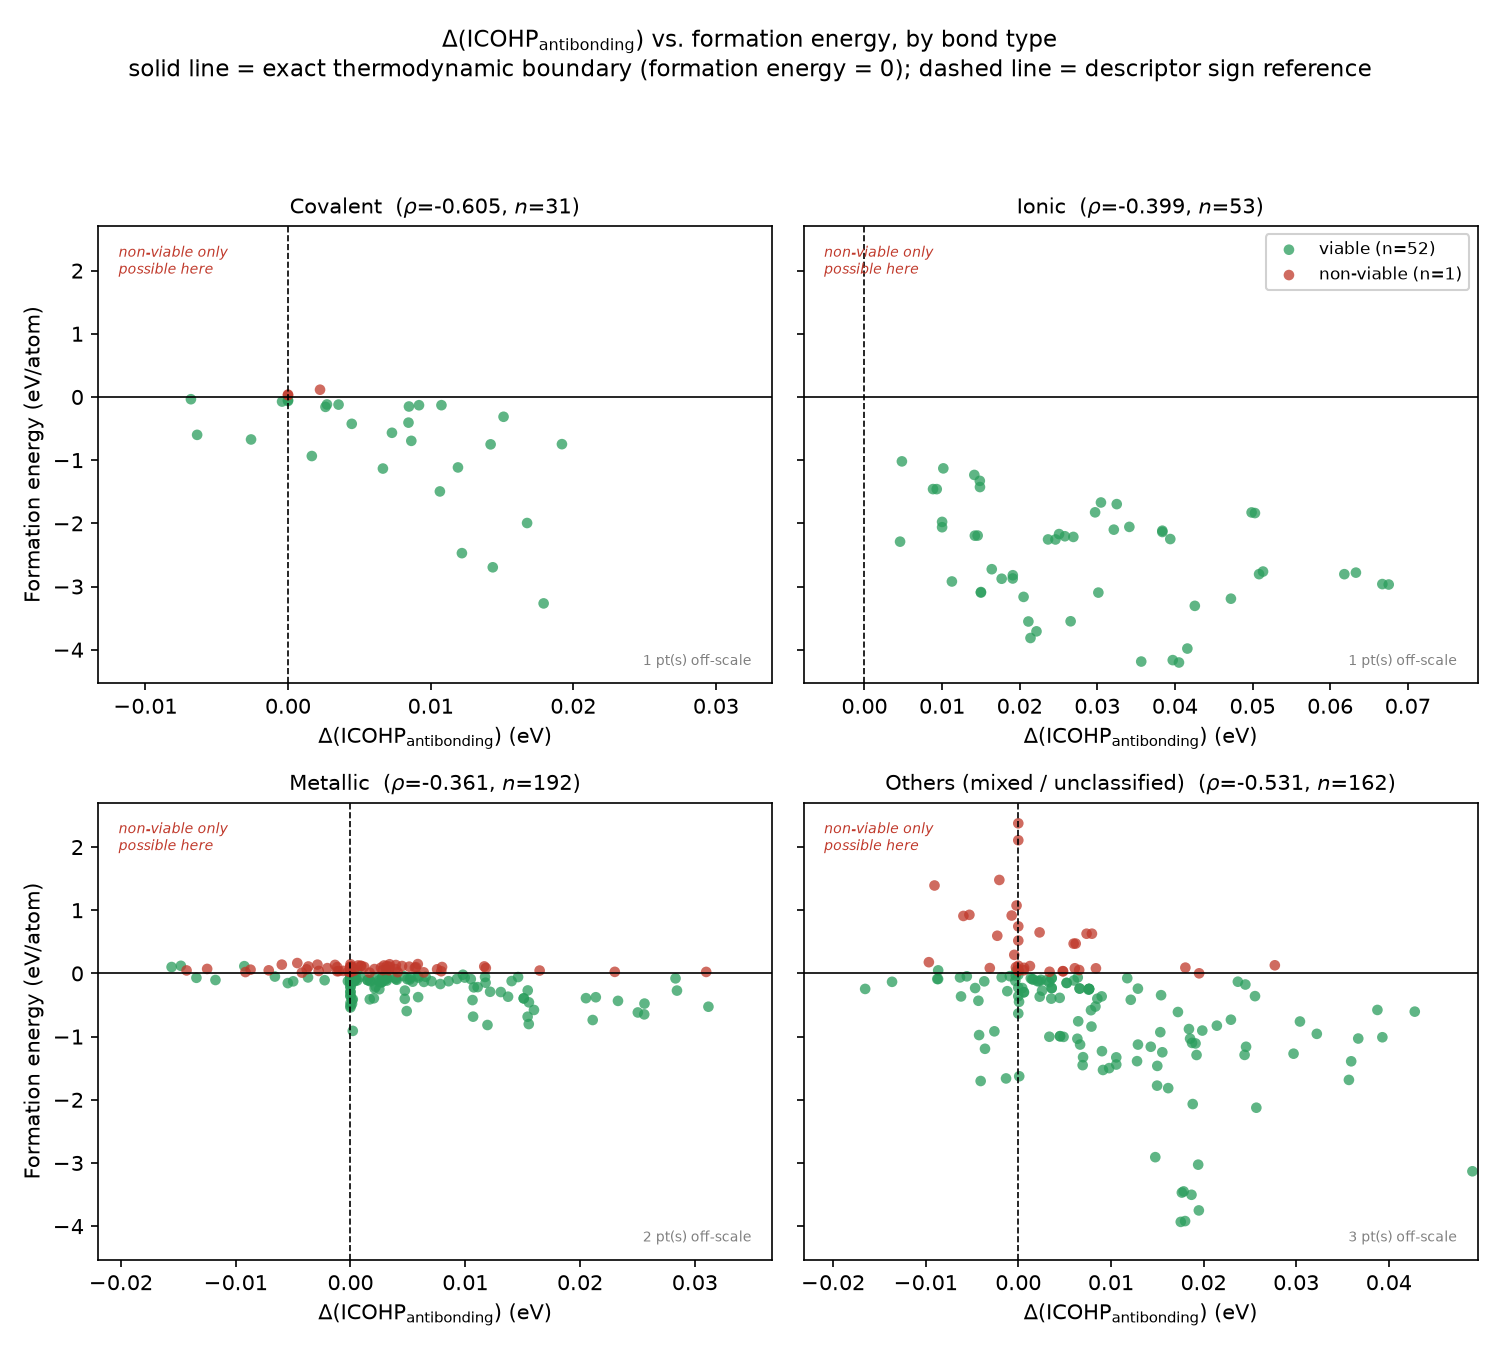
\includegraphics[width=0.9\textwidth]{antibonding_viability_by_bondtype.png}
\caption{Formation energy versus $\Delta$(ICOHP\textsubscript{antibonding})
by \texttt{bond\_type} subgroup, colored by \texttt{ViabilityLabel}
(viable~$=$~\texttt{STABLE\_ON\_HULL}~$\cup$~\texttt{METASTABLE\_VIABLE},
non-viable~$=$~\texttt{UNSTABLE\_NONEXISTENT}). The solid horizontal line
(formation energy~$=0$) is the exact, descriptor-independent half of the
\texttt{classify\_viability()} boundary: every compound at or below it is
\texttt{STABLE\_ON\_HULL} regardless of bonding. The dashed vertical line
marks $\Delta$(ICOHP\textsubscript{antibonding})~$=0$, the sign tested in
Table~\ref{tab:viability-antibonding} --- not itself the literal
\texttt{classify\_viability()} boundary, which is defined on the total
reaction $\Delta$(ICOHP) of Section~\ref{sec:delta-icohp} rather than its
antibonding-only counterpart. Non-viable compounds separate cleanly from
viable ones in the ionic and mixed/unclassified subgroups but overlap the
sign boundary in the metallic subgroup, consistent with
\texttt{bond\_type}=metallic being the one subgroup that does not reach
significance in Table~\ref{tab:viability-antibonding}. A handful of
extreme-magnitude compounds per panel are clipped from the visible range
(count noted in-panel); axis limits therefore differ between panels.}
\label{fig:antibonding-viability-by-bondtype}
\end{figure}

A compound whose formation reduces near-frontier antibonding character
relative to its constituent elements is significantly more likely to be
classified viable than one whose formation increases it --- overall and
within every subgroup large enough to test, including
\texttt{is\_metal}=False despite its thin non-viable class (only 6
compounds). Combined with the stratification result of
Section~\ref{sec:res-stratification}, this gives two independent lines of
evidence --- a continuous thermodynamic correlate and a categorical
viability test --- pointing the same way: reduced near-$E_\text{F}$
antibonding character upon formation tracks not only how thermodynamically
favorable a compound's formation is, but which compounds actually persist.

\subsection{Polymorph Comparison}
\label{sec:res-polymorph}

Sections~\ref{sec:res-baseline}--\ref{sec:res-viability} test whether the
antibonding descriptor distinguishes a compound from its own elements. A
distinct question, motivated by the dataset's own design
(Section~\ref{sec:dataset}, track (ii), built specifically ``to build
genuine same-composition polymorph groups and to probe descriptor
behavior far from equilibrium''), is whether it distinguishes the more
stable of two polymorphs of the \emph{same} composition from each other
--- the antibonding-descriptor analog of the fully integrated reaction
$\Delta$(ICOHP)'s own polymorph test (Case 2, 47.3\% agreement between
most-bonding and most-stable member, statistically indistinguishable
from the 42.4\% chance baseline). Every \texttt{icobi\_label} bond-type
group with at least one same-formula group of size $\geq2$ (duplicate
\texttt{mp\_id} entries under inconsistent naming removed first) is
tested independently: Spearman $\rho$ between each of the raw ICOHP- and
ICOBI-based antibonding populations and each polymorph's enthalpy above
its own group's most stable member ($\Delta H$), and, where a case-1
reaction is available for enough of the group, the same test against
each reaction $\Delta$(antibonding). ICOBI is tested alongside ICOHP
throughout this work (never in isolation); their raw populations run in
formally opposite sign conventions (Section~\ref{sec:antibonding-def})
but that does not by itself predict whether the two behave alike on this
polymorph-ranking question, which is why both are reported rather than
assuming one mirrors the other.

\begin{table}[htbp]
\centering
\caption{Spearman correlation between each antibonding descriptor and
same-formula polymorph enthalpy ($\Delta H$ above the group's own most
stable member), by \texttt{icobi\_label} bond-type group.}
\label{tab:polymorph-antibonding}
\begin{tabular}{@{}lrrrrrrrrrrrr@{}}
\toprule
& \multicolumn{6}{c}{ICOHP-based} & \multicolumn{6}{c}{ICOBI-based} \\
& \multicolumn{3}{c}{Raw} & \multicolumn{3}{c}{Reaction $\Delta$} & \multicolumn{3}{c}{Raw} & \multicolumn{3}{c}{Reaction $\Delta$} \\
Group & $n$ & $\rho$ & $p$ & $n$ & $\rho$ & $p$ & $n$ & $\rho$ & $p$ & $n$ & $\rho$ & $p$ \\
\midrule
Ionic (25) & 53 & $-0.089$ & $0.53$ & 48 & $-0.008$ & $0.96$ & 53 & $-0.115$ & $0.41$ & 48 & $+0.040$ & $0.79$ \\
Covalent (6) & 20 & $-0.206$ & $0.38$ & 8 & $-0.172$ & $0.68$ & 20 & $+0.141$ & $0.55$ & 8 & $-0.158$ & $0.71$ \\
Mixed (10) & 24 & $+0.079$ & $0.72$ & 9 & $-0.322$ & $0.40$ & 24 & $+0.360$ & $0.084$ & 9 & $+0.094$ & $0.81$ \\
Metallic (27) & 62 & $+0.114$ & $0.38$ & 39 & $-0.207$ & $0.21$ & 62 & $-0.073$ & $0.57$ & 39 & $+0.104$ & $0.53$ \\
\bottomrule
\end{tabular}
\vspace{0.1cm}
\\{\footnotesize Number of same-formula groups per bond type in
parentheses.}
\end{table}

\begin{figure}[htbp]
\centering
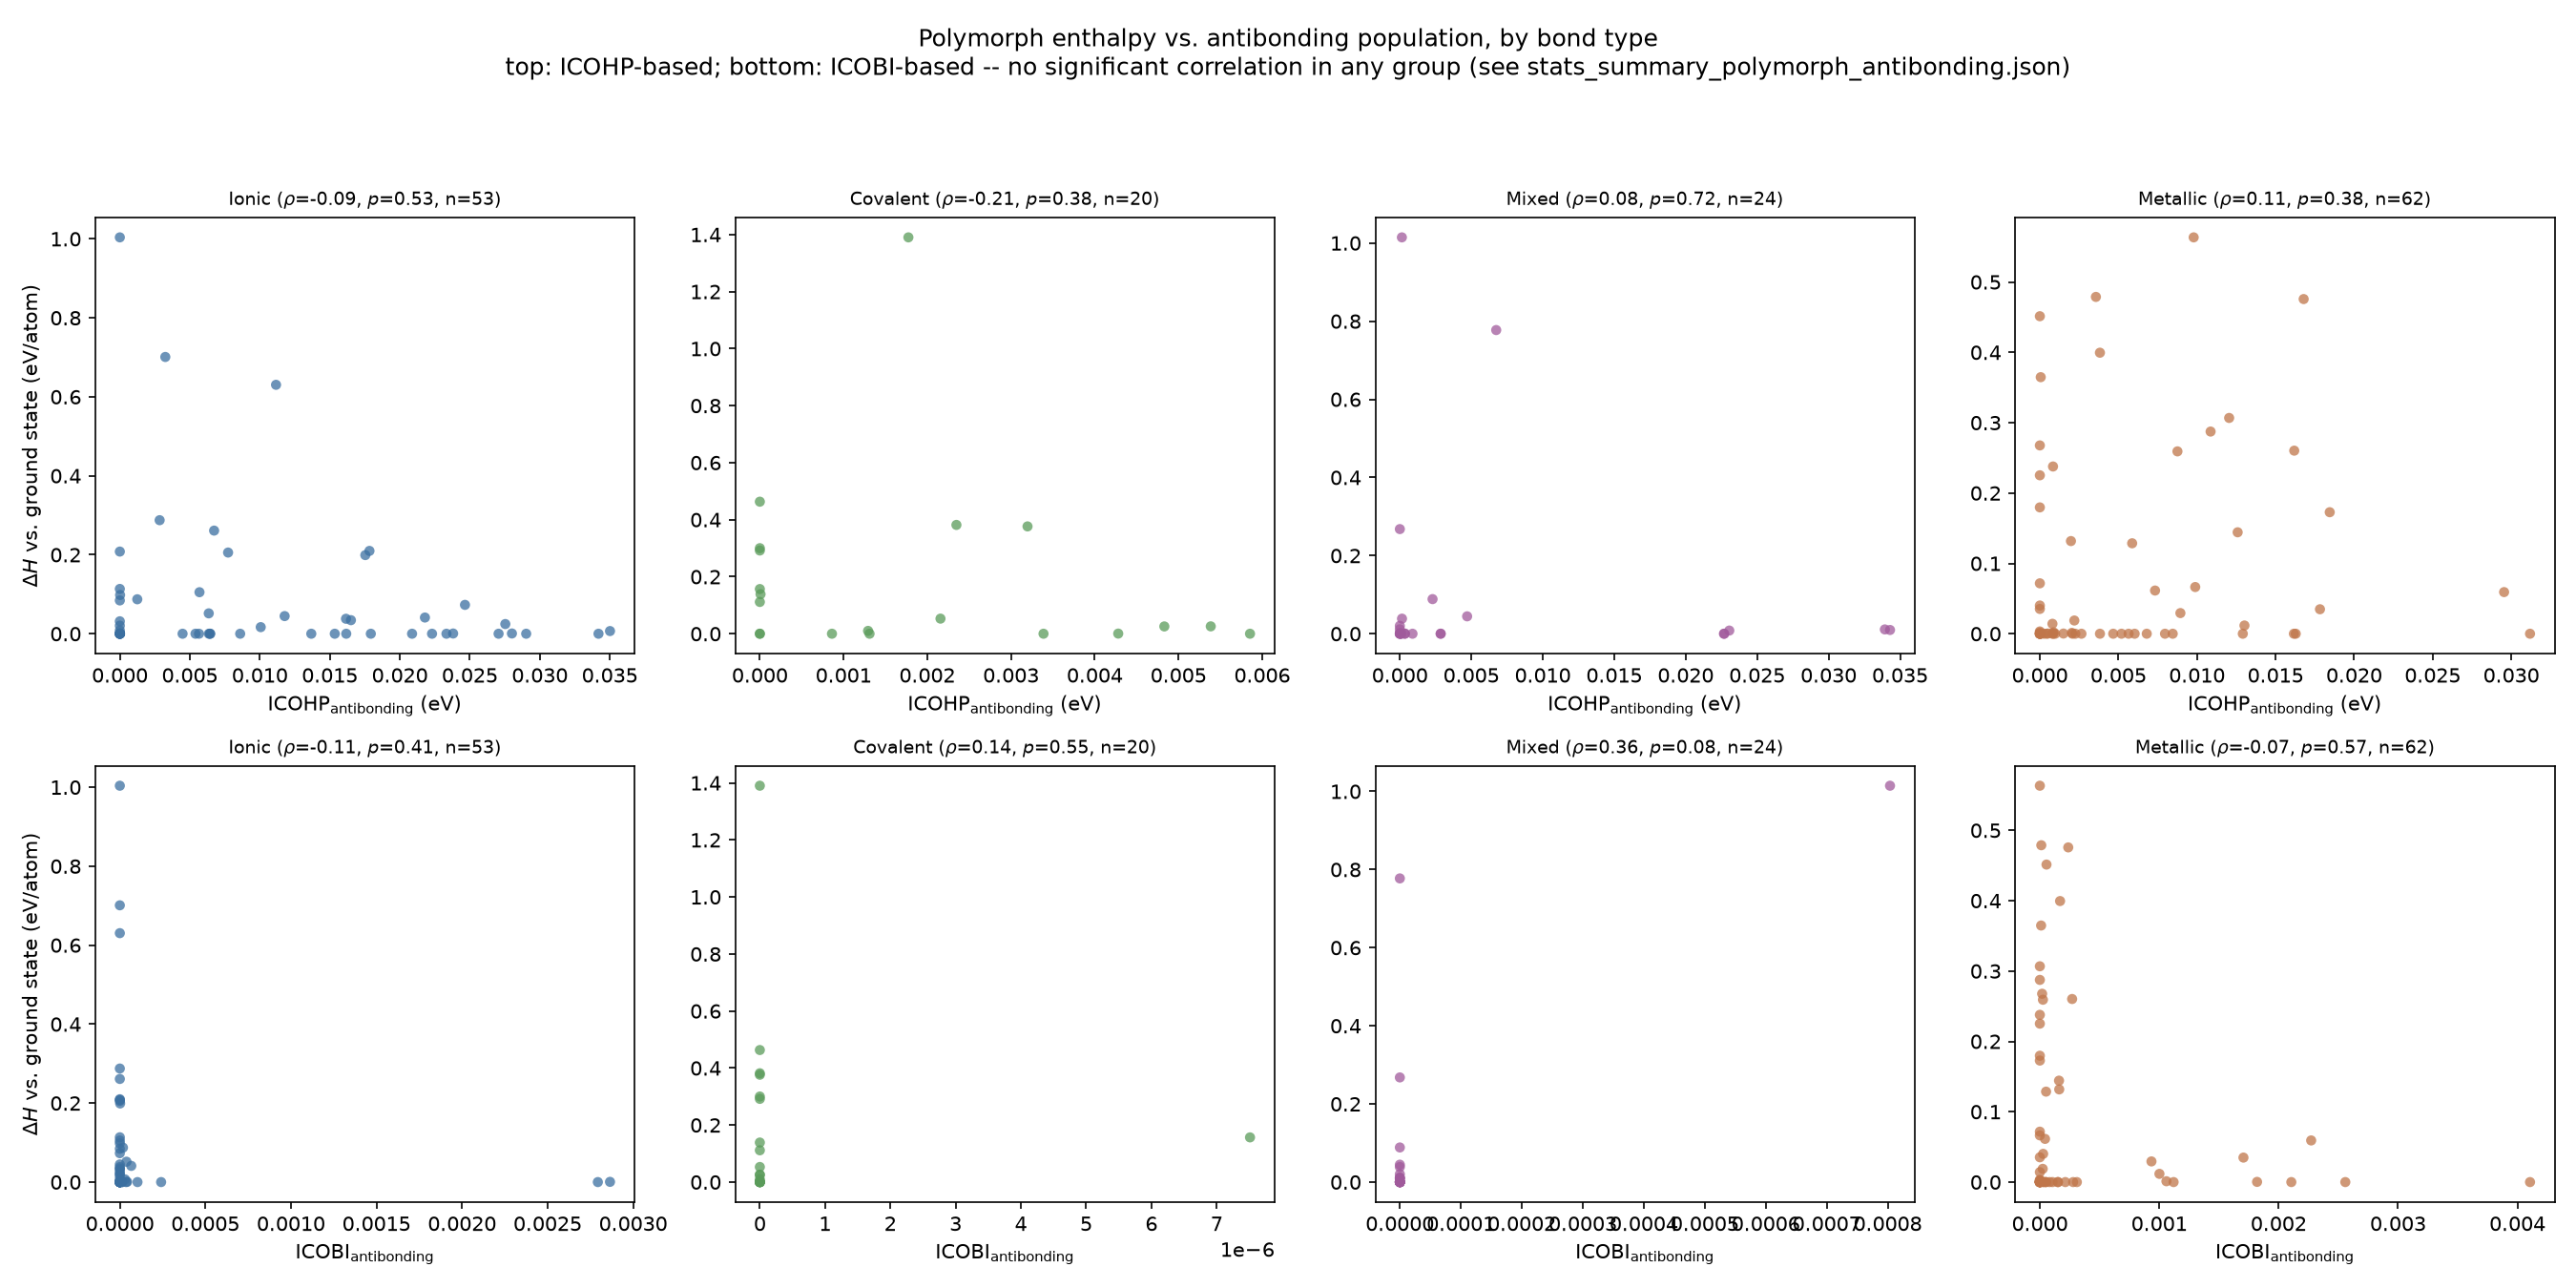
\includegraphics[width=\textwidth]{polymorph_antibonding_correlation.png}
\caption{Polymorph enthalpy above the same-formula ground state versus
raw antibonding population, one column per \texttt{icobi\_label}
bond-type group, ICOHP-based (top row) and ICOBI-based (bottom row).}
\label{fig:polymorph-antibonding}
\end{figure}

No group reaches significance, for either descriptor or either the raw
or the reaction construction ($p>0.2$ throughout except two borderline
cases still short of the conventional threshold: ionic's raw ICOHP
result restricted to non-ground-state members only, $p=0.068$, and
mixed's raw ICOBI result, $p=0.084$, $n=24$ formulas/rows only). This
mirrors the fully integrated reaction $\Delta$(ICOHP)'s own Case 2
result exactly: whatever makes the antibonding descriptors effective
viability pre-screens against a compound's own elements
(Sections~\ref{sec:res-baseline}--\ref{sec:res-viability}) does not carry
over to ranking polymorphs of a fixed composition against each other ---
a genuinely different comparison (same reactants, different local
bonding topology) rather than a restatement of the same test at smaller
scale.

\subsection{Discussion}
\label{sec:res-discussion}

Three findings, taken together, motivate treating
$\Delta$(ICOBI\textsubscript{antibonding}) --- and its ICOHP counterpart,
reported throughout for comparison --- as a genuine viability pre-screen
rather than a restatement of formation energy under a different name. First,
restricting the antibonding integration to a narrow window adjacent to the
Fermi level (or the valence-band maximum) and taking its reaction $\Delta$
consistently outperforms both the classic ICOHP aggregates and the fully
integrated reaction $\Delta$(ICOHP) baseline (Section~\ref{sec:res-baseline}),
and does so for both the ICOHP- and the ICOBI-based construction, despite
their raw (non-reaction) versions running in formally opposite directions.
Second, unlike every other descriptor tested in this work, the reaction
$\Delta$(antibonding) construction survives stratification by bonding type
in \emph{every} subgroup large enough to test (Section~\ref{sec:res-stratification})
--- metallic, ionic, covalent, and mixed alike --- rather than being carried
by one dominant chemical class or flipping sign across strata, as the fully
integrated reaction $\Delta$(ICOHP) does (ionic positive, covalent/mixed
negative; Section~\ref{sec:res-baseline}). Third, it discriminates
experimentally realized from theoretical-only compounds directly
(Section~\ref{sec:res-viability}), not merely via a correlation with a
continuous thermodynamic proxy for that status.

This combination of properties is what makes
$\Delta$(ICOBI\textsubscript{antibonding}) attractive specifically as a
pre-screen ahead of the phonon/elastic/AIMD stability hierarchy described in
Section~\ref{sec:intro}: it requires nothing beyond the single static
DFT+LOBSTER calculation already described in
Section~\ref{sec:dft-lobster} --- no supercell, no finite-strain set, no
finite-temperature trajectory --- and, being a bond-order-based rather than
a total-energy-based quantity, it is available immediately alongside a
compound's ICOHP/ICOBI bonding characterization rather than requiring an
additional calculation. For a CSP campaign generating far more metastable
stationary points than can be individually subjected to phonon or AIMD
screening, ranking candidates by $\Delta$(ICOBI\textsubscript{antibonding})
offers a physically motivated way to concentrate that downstream budget on
the candidates most likely to correspond to kinetically persistent,
isolable compounds.

Some caveats temper this picture. The descriptor is validated here on a
single dataset assembled specifically to span the stability spectrum
(Section~\ref{sec:dataset}), including a deliberately adversarial subset of
theoretical polymorphs selected to sit far above the convex hull; whether
the viability discrimination of Section~\ref{sec:res-viability} partly
reflects that selection choice rather than being an independent confirmation
of the underlying bonding-kinetics mechanism has not yet been fully
disentangled, and is a direct target for the independent-dataset test
proposed in Section~\ref{sec:conclusion}. The \texttt{theoretical}-only
status used to define ``not viable'' throughout is itself a proxy --- the
absence of a synthesis report, not a measured kinetic barrier or a
phonon-instability verdict --- and several of this project's smaller
bonding-type subgroups (Table~\ref{tab:delta-antibonding-stratified})
remain modest in size. Finally, because the fully integrated reaction
$\Delta$(ICOHP) changes sign across bonding-type strata
(Section~\ref{sec:res-baseline}), any future symbolic-regression or
feature-selection search built on these descriptors should be run separately
per bonding type rather than on the pooled population, where such a search
would risk being actively misleading.

\subsection{Current Limits}
\label{sec:limits}

A systematic sweep of the dataset flagged a single compound (a
copper--gold intermetallic) for exclusion from every statistic reported
above: its LOBSTER projection fails $k$-point orthonormalization at 100\% of
sampled $k$-points, with a maximum \texttt{bandOverlaps.lobster} deviation of
11.4 against this project's own 0.1 red-flag threshold (Section~\ref{sec:validation-methods}),
and correspondingly implausible ICOHP values (third-neighbor contacts with
positive ICOHP an order of magnitude too large to be physical). The
next-worst case in the full 597-structure sweep is already
29$\times$ less extreme and plausibly reflects genuine, dense
$d$-electron-rich intermetallic chemistry rather than a projection failure,
confirming the excluded compound as a unique quality-control case rather
than a symptom of a broader problem; every statistic in this article has
been computed on the remaining structures.

Beyond this single exclusion, three further limitations bound the scope of
the present analysis. First, the \texttt{theoretical}-only proxy for
non-viability, discussed above, is not a true dynamical-instability label;
extending the dataset with explicit phonon calculations for a representative
subset would allow $\Delta$(ICOBI\textsubscript{antibonding}) to be tested
against a genuinely independent stability criterion rather than against
synthesis history alone. Second, per-subgroup sample size remains this
project's structural limit at every new stratification: the raw antibonding
population's covalent-subgroup result reported at $n=33$ in an earlier,
smaller version of this dataset ($\rho=-0.551$) did not survive once the
sample grew to $n=54$ ($\rho=-0.046$; Section~\ref{sec:res-baseline}), a
concrete illustration that any single-stratum result should be re-checked as
a dataset grows rather than accepted once and for all. Third, because
reaction $\Delta$(ICOHP)'s signal changes sign across bonding-type strata
(Section~\ref{sec:res-discussion}), a pooled symbolic-regression search
(e.g. SISSO) across the whole dataset is deferred in favor of a future
per-bonding-type search, left to subsequent work.

\section{Conclusion}
\label{sec:conclusion}

Restricting the integration of the ICOHP and ICOBI bonding-population traces
to a narrow, one-sided window adjacent to the Fermi level (or the
valence-band maximum), and referencing the resulting near-frontier
antibonding population against a compound's own constituent elements
through the reaction quantity $\Delta$(antibonding) (Eq.~\ref{eq:delta-antibonding}),
yields the most robust viability descriptor identified in this work.
$\Delta$(ICOBI\textsubscript{antibonding}) correlates significantly with
formation energy ($\rho=-0.429$, $n=438$), survives stratification by
bonding type in every subgroup tested --- a property no other descriptor in
this study shares, including the fully integrated reaction
$\Delta$(ICOHP) and the raw (non-reaction) antibonding population --- and,
alongside its ICOHP-based counterpart, significantly discriminates
experimentally realized from theoretical-only metastable compounds
(Fisher's exact test, $p=2.4\times10^{-7}$, overall). Because it is obtained
from the same single static DFT+LOBSTER calculation already required to
characterize a compound's bonding, it offers a computationally inexpensive
pre-screen for kinetic viability, to be applied ahead of the far more
costly phonon, elastic-constant, and AIMD stages of the stability hierarchy
outlined in Section~\ref{sec:intro}, concentrating that downstream budget on
the metastable CSP candidates most likely to correspond to isolable
compounds.

Three directions follow directly from the limitations noted in
Section~\ref{sec:limits}. First, reproducing the present correlations and
stratified results on an independently assembled dataset, ideally one not
built with the current dataset's deliberately adversarial, far-above-hull
theoretical subset, would distinguish a genuine bonding-kinetics mechanism
from a residual selection effect. Second, testing
$\Delta$(ICOBI\textsubscript{antibonding}) against explicit phonon and
elastic-constant calculations for a representative subset would replace the
synthesis-history proxy used here with a directly computed dynamical
criterion. Third, a bonding-type-resolved symbolic-regression search (e.g.
SISSO), run separately per stratum rather than on the pooled population,
could clarify whether $\Delta$(ICOBI\textsubscript{antibonding}) can be
combined with complementary descriptors --- or refined into a still sharper
one --- within each chemical class; extending the underlying dataset to
ternary and higher-order chemistry, and to explicit pressure dependence in
line with the high-pressure CSP context of Section~\ref{sec:intro}, are
natural companions to that effort.

\begin{acknowledgement}
\textit{Acknowledgements and funding sources to be added.}
\end{acknowledgement}

\paragraph{Data Availability.} The dataset, computational scripts, and
analysis code underlying this article are available in the project's
repository (URL to be finalized for publication).

\begin{suppinfo}
Dataset composition and selection criteria; complete list of the compounds
and elements studied; VASP and LOBSTER input parameters (INCAR, POTCAR, and
$k$-point grids); LOBSTER quality-control diagnostics for the full dataset;
the complete list of case-1
decomposition-into-elements reactions with $\Delta$(ICOHP),
$\Delta$(ICOHP\textsubscript{antibonding}), and
$\Delta$(ICOBI\textsubscript{antibonding}) values; endobondic and exobondic
reaction subsets.
\end{suppinfo}

\bibliography{references}

\end{document}
